\chapter{Simulazione di una coda $M/G/1$}
\label{ch:mg1}

\section{Sistema a coda $M/G/1$}

Il sistema considerato in questo capitolo \`e di tipo a singolo servitore, con arrivi di tipo poissoniano, tempi di servizio variabilmente distribuiti e media $\mu$ definiti dall'utente in fase di inizializzazione.

\begin{figure}[!h]{
	\begin{center}
	   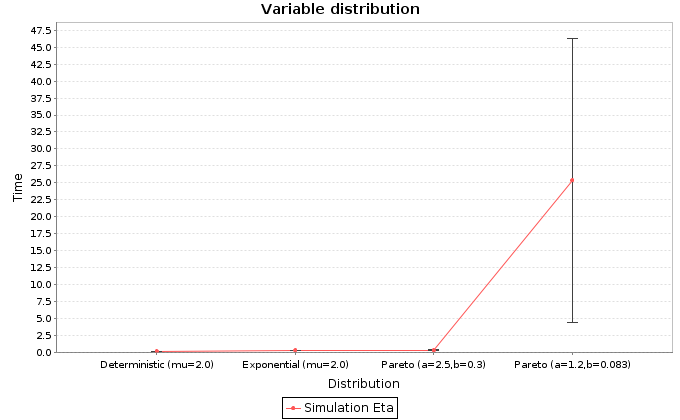
\includegraphics[width=\textwidth]{figures/mg1dists.png}
	\end{center}}
	\caption{Tempi medi di attesa al variare del tipo di distribuzione $\rho=0.4$, $\mu=2.0$, $N=100$}
	\label{fig:mg1dists}
\end{figure}

\begin{figure}[!h]{
	\begin{center}
	   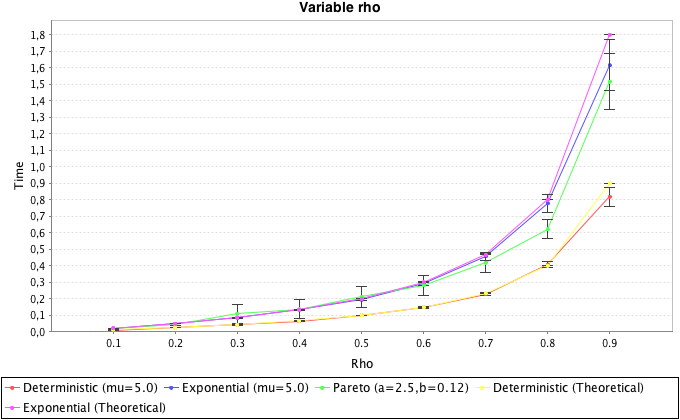
\includegraphics[width=\textwidth]{figures/cfrdists.png}
	\end{center}}
	\caption{Tempi medi di attesa al variare di $\rho$ per i vari tipi di distribuzione}
	\label{fig:cfrdists}
\end{figure}

La simulazione di una coda di tipo $M/G/1$ pu\`o essere effettuata, come da specifica richiesta, in funzione delle varie tipologie di distribuzione o in funzione della variazione supervisionata di $\rho$ nell'intervallo $(0,1)$.

\begin{figure}[!h]{
	\begin{center}
	   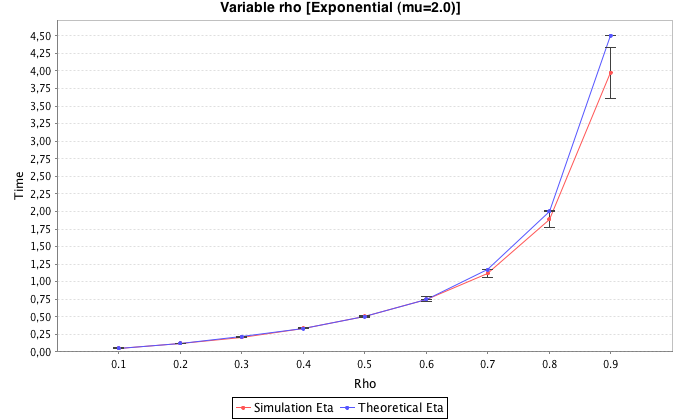
\includegraphics[width=\textwidth]{figures/mg1expmu2.png}
	\end{center}}
	\caption{Tempi medi di attesa al variare di $\rho$ con distribuzione Poissoniana dei tempi di servizio}
	\label{fig:mg1expmu2}
\end{figure}

\begin{figure}[!h]{
	\begin{center}
	   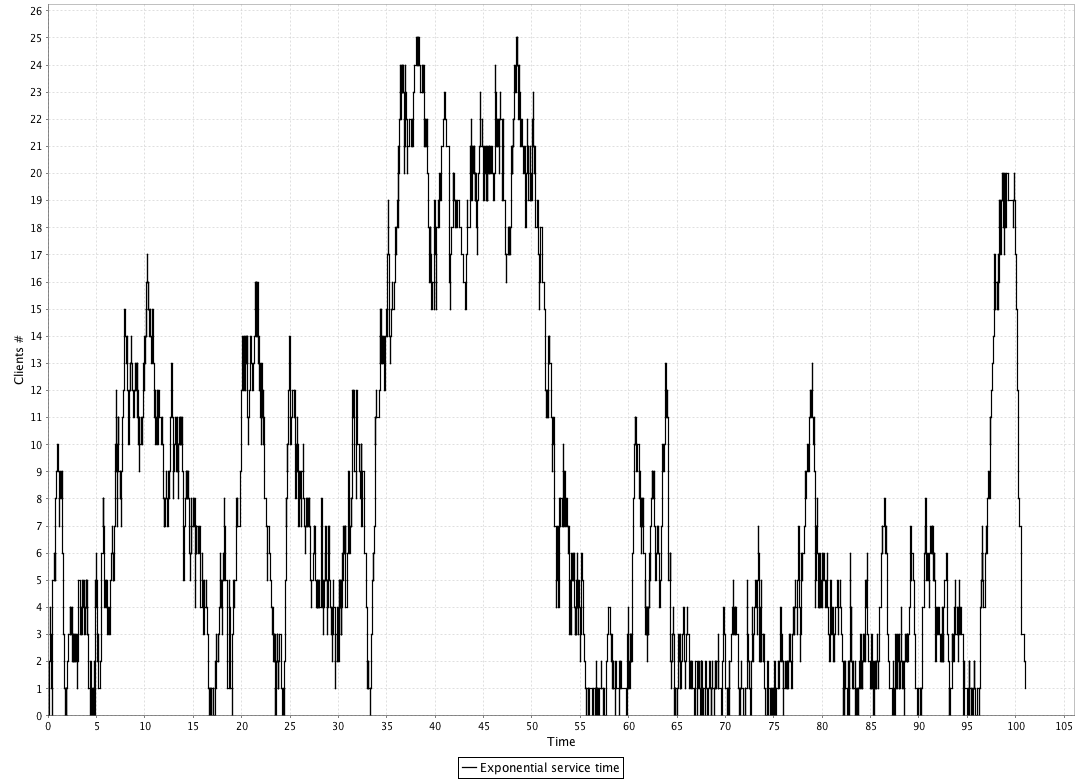
\includegraphics[width=\textwidth]{figures/kt.png}
	\end{center}}
	\caption{Numero di utenti nel sistema $k(t)$ in funzione del tempo, durante una simulazione}
	\label{fig:kt}
\end{figure}

La simulazione in funzione della tipologia di distribuzione permette di apprezzare, analogamente a quanto visto in fase di analisi teorica, come la distribuzione di Pareto configurata con parametro $1<\alpha\le2$ presenti un'estrema variabilit\`a, soprattutto se postaa confronto con traffico di tipo Poissoniano o deterministico (figura \ref{fig:mg1dists}).

La simulazione in funzione della variazione di $\rho$\footnote{la simulazione \`e stata realizzata facendo variare $\rho$ nell'intervallo $[0.1, 0.9]$ con passo di incremento pari a $0.1$} evidenzia la tendenza a divergere del tempo medio di attesa nel sistema $\eta$ al crescere dell'occupazione dell'unico servitore presente. In figura \ref{fig:mg1expmu2} \`e possibile notare come la caratterizzazione qualitativa e quantitativa dei dati ricalchi in maniera molto fedele l'andamento della curva teorica relativa ai sistemi $M/G/1$.

All'interno della scheda dedicata alla simulazione della coda $M/G/1$ \`e possibile notare l'opzione relativa alla stima della probabilit\`a di stato della coda, tale opzione \`e parte delle simulazioni a scelta implementate e verr\`a meglio esposta al capitolo \ref{ch:optional}.


\subsection{Analisi tecnica}

La struttura del simulatore \`e stata definita in aderenza alle specifiche fornite all'interno delle slide a supporto del corso \cite{cerroni01}. 
Al fine aggiuntivo di conferire al sistema una migliore strutturazione dal punto di vista dell'ingegneria del software si \`e deciso di implementare una classe astratta {\tt Simulator}, svincolata dalla specifica politica di gestione delle code utilizzata. 

Tale polica viene infatti gestita specificamente all'interno di due specializzazioni della suddetta classe, tali {\tt FCFSSimulator} e {\tt SJNSimulator}, che nell'ordine realizzano un simulatore in cui la politica di servizio \`e \emph{``first-come/first-served''} e \emph{``shortest-job next''}.

La gestione della simulazione viene, in fase preliminare, gestita all'interno del pannello dell'interfaccia grafica dedicato. Dopo l'analisi della correttezza dell'input per\`o, al fine di garantire il massimo disaccoppiamento tra elborazione dati e interazione con l'utente, viene generato un nuovo thread che tramite l'utilizzo di metodi dedicati della classe {\tt SimulationRunners} permette lo svolgimento effettivo della simulazione. Al termine di quest'ultima verranno quindi generati eventuali grafici e/o output in console.

\begin{figure}[!h]{
	\begin{center}
	   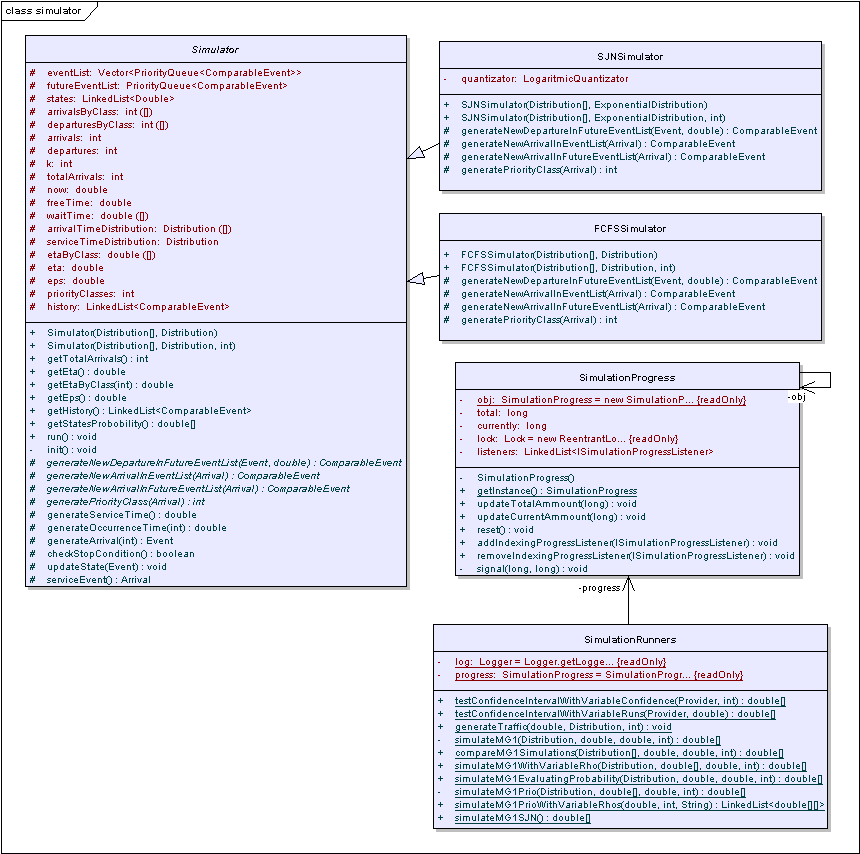
\includegraphics[width=\textwidth]{figures/simulatorclass.png}
	\end{center}}
	\caption{Struttura del package {\tt simulator}}
	\label{fig:simulatorclass}
\end{figure}

Un'ulteriore accorgimento messo in atto per evitare l'andarsi a delineare di situazione di forte concorrenza in fase di esecuzione\footnote{vista anche la grande richiesta computazionale in fase di simulazione, determinata da una sostanziale prevalenza di cicli cpu-burst.} \`e il ricorso alla classe {\tt ExecutorService}. In particolare, l'esecuzione delle simulazioni viene in tutte le sue forme demandata ad un istanza della classe {\tt ExecutorService} instanziata attraverso l'invocazione del costruttore {\tt newSingleThreadExecutor()} della classe {\tt Executor}, che di fatto permette l'utilizzo controllato di un singolo thread per le operazioni a maggior carico computazionale.

In figura \ref{fig:simulatorclass} \`e possibile osservare la strutturazione definita per entit\`a dedicate alla simulazione.

